In order to see the big picture, we decided to use an approach from Cadle\&Yeates\cite{caye} known as a \emph{work breakdown structure}. The work breakdown structure is organized in a hierarchical tree structure, where each new level in the tree is created by dividing a task into subtasks, as shown in figure \ref{fig:breakdown}.

\begin{figure}[hbtp]
	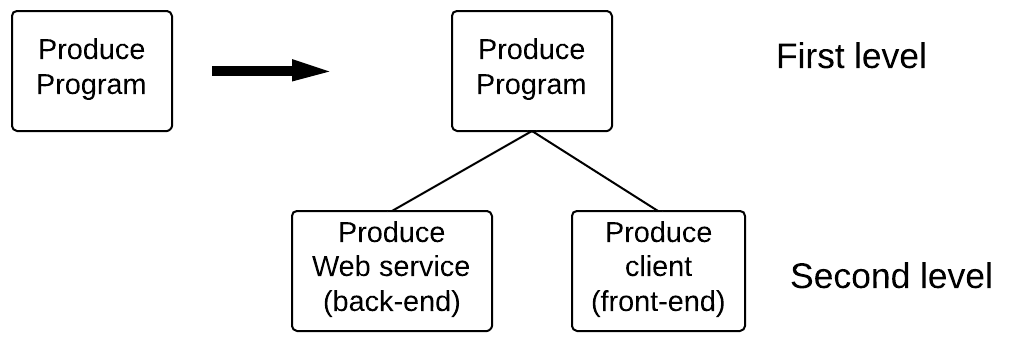
\includegraphics[scale=0.5]{./Empiri/Planning/img/wbslevels.png}
	\caption{Example work breakdown structure} \label{fig:breakdown}
\end{figure}

The division of tasks into smaller components is an iterative process, which stops when the resulting tasks are small enough to be considered a suitable assignment for one man or, more subjectively, when it simply does not make sense to divide it any further.

Our work breakdown structure can be found in appendix \ref{app:workbreak}.